\documentclass{article}
\usepackage[T1,T2A]{fontenc}
\usepackage[utf8]{inputenc}
\usepackage[english,ukrainian]{babel}
\usepackage[]{amsthm} %lets us use \begin{proof}
\usepackage[]{amssymb} %gives us the character \varnothing
\usepackage{graphicx}

\begin{document}

\title{Домашка 5. Відображення і графи}
\date{30 травня 2023}

\maketitle

\subsection*{Задача 1}
Чи є наступні функції інєкцією, сурєкцією, бієкцією. Доведіть або приведіть контрприклад
\begin{itemize}
    \item $f: \mathbb{R} \setminus \{0\} \rightarrow \mathbb{R} f(x)=\frac{3x-1}{x}$
    \item $f: \mathbb{R} \setminus \{1\} \rightarrow \mathbb{R} \setminus \{1\} f(x)=\frac{x+1}{x-1}$
    \item $f: \mathbb{R} \rightarrow \mathbb{R} f(x)=x^4$
    \item $f: \mathbb{R}^+ \rightarrow \mathbb{R}^+ f(x)=x^4$
    \item $X=\{a,b,c,d\} A=\mathcal{P}(X) f: A \rightarrow \{0,1,2,3,4\} f(x) = |x|$
\end{itemize}

\subsection*{Задача 2}
Намалюйте граф або доведіть, що його не існує
\begin{itemize}
    \item З 5 вершинами і степенями 1,2,3,4,5
    \item З 6 вершинами і степенями 1,2,3,4,5,6
    \item Простий граф з 5 вершинами і степенями 1,1,3,4,5
    \item Граф у якому немає циклів
    \item Зв'язний граф у якому немає циклів
    \item Граф у якому є ейлерів цикл, але немає гамільтонового
    \item Граф у якому є гамільтонів цикл, але немає ейлерового
\end{itemize}

\subsection*{Задача 3}
Для наступних графів знайдіть Ейлеровий цикл та шлях, Гамільтонів цикл, або доведіть, що їх немає
\pagebreak

\begin{figure}
\centering
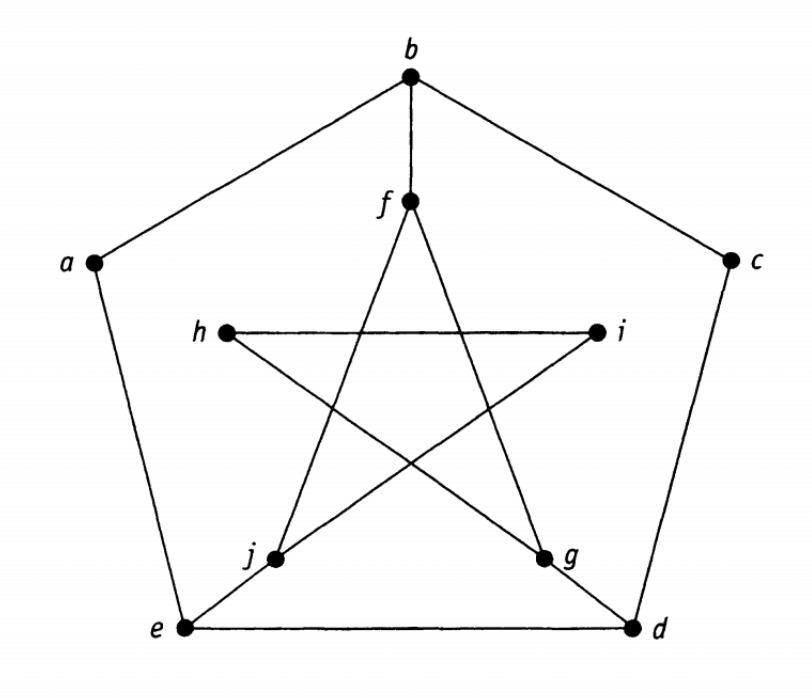
\includegraphics[width=90mm]{h1}
\end{figure}

\begin{figure}
\centering
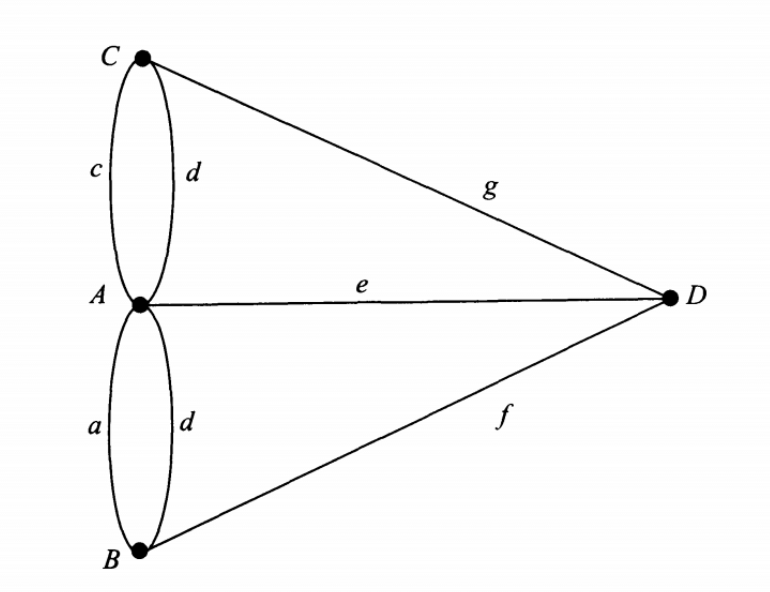
\includegraphics[width=90mm]{h2}
\end{figure}

\begin{figure}
\centering
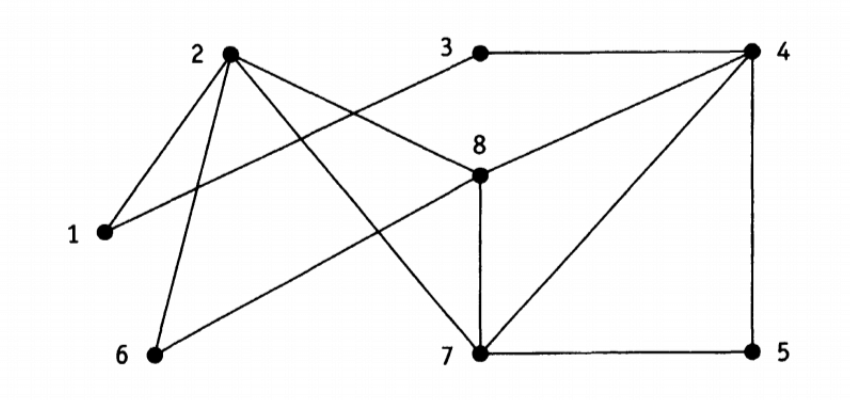
\includegraphics[width=90mm]{h3}
\end{figure}

\begin{figure}
\centering
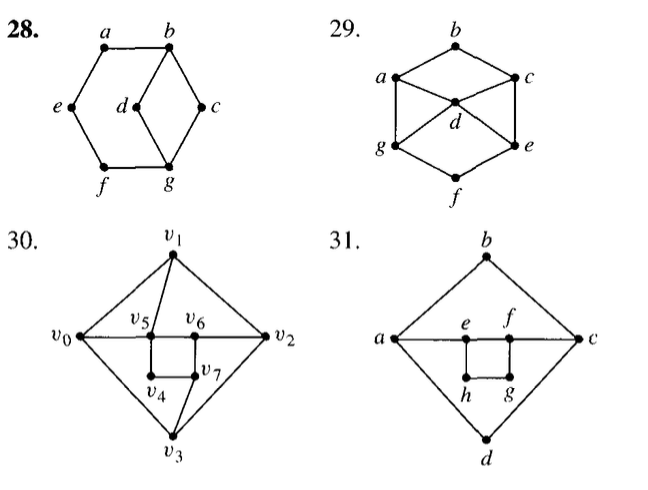
\includegraphics[width=90mm]{h4}
\end{figure}

\end{document}